\newpage
\section*{Introduction}
\label{sec:intros}
% \begin{figure}
%     \centering
%     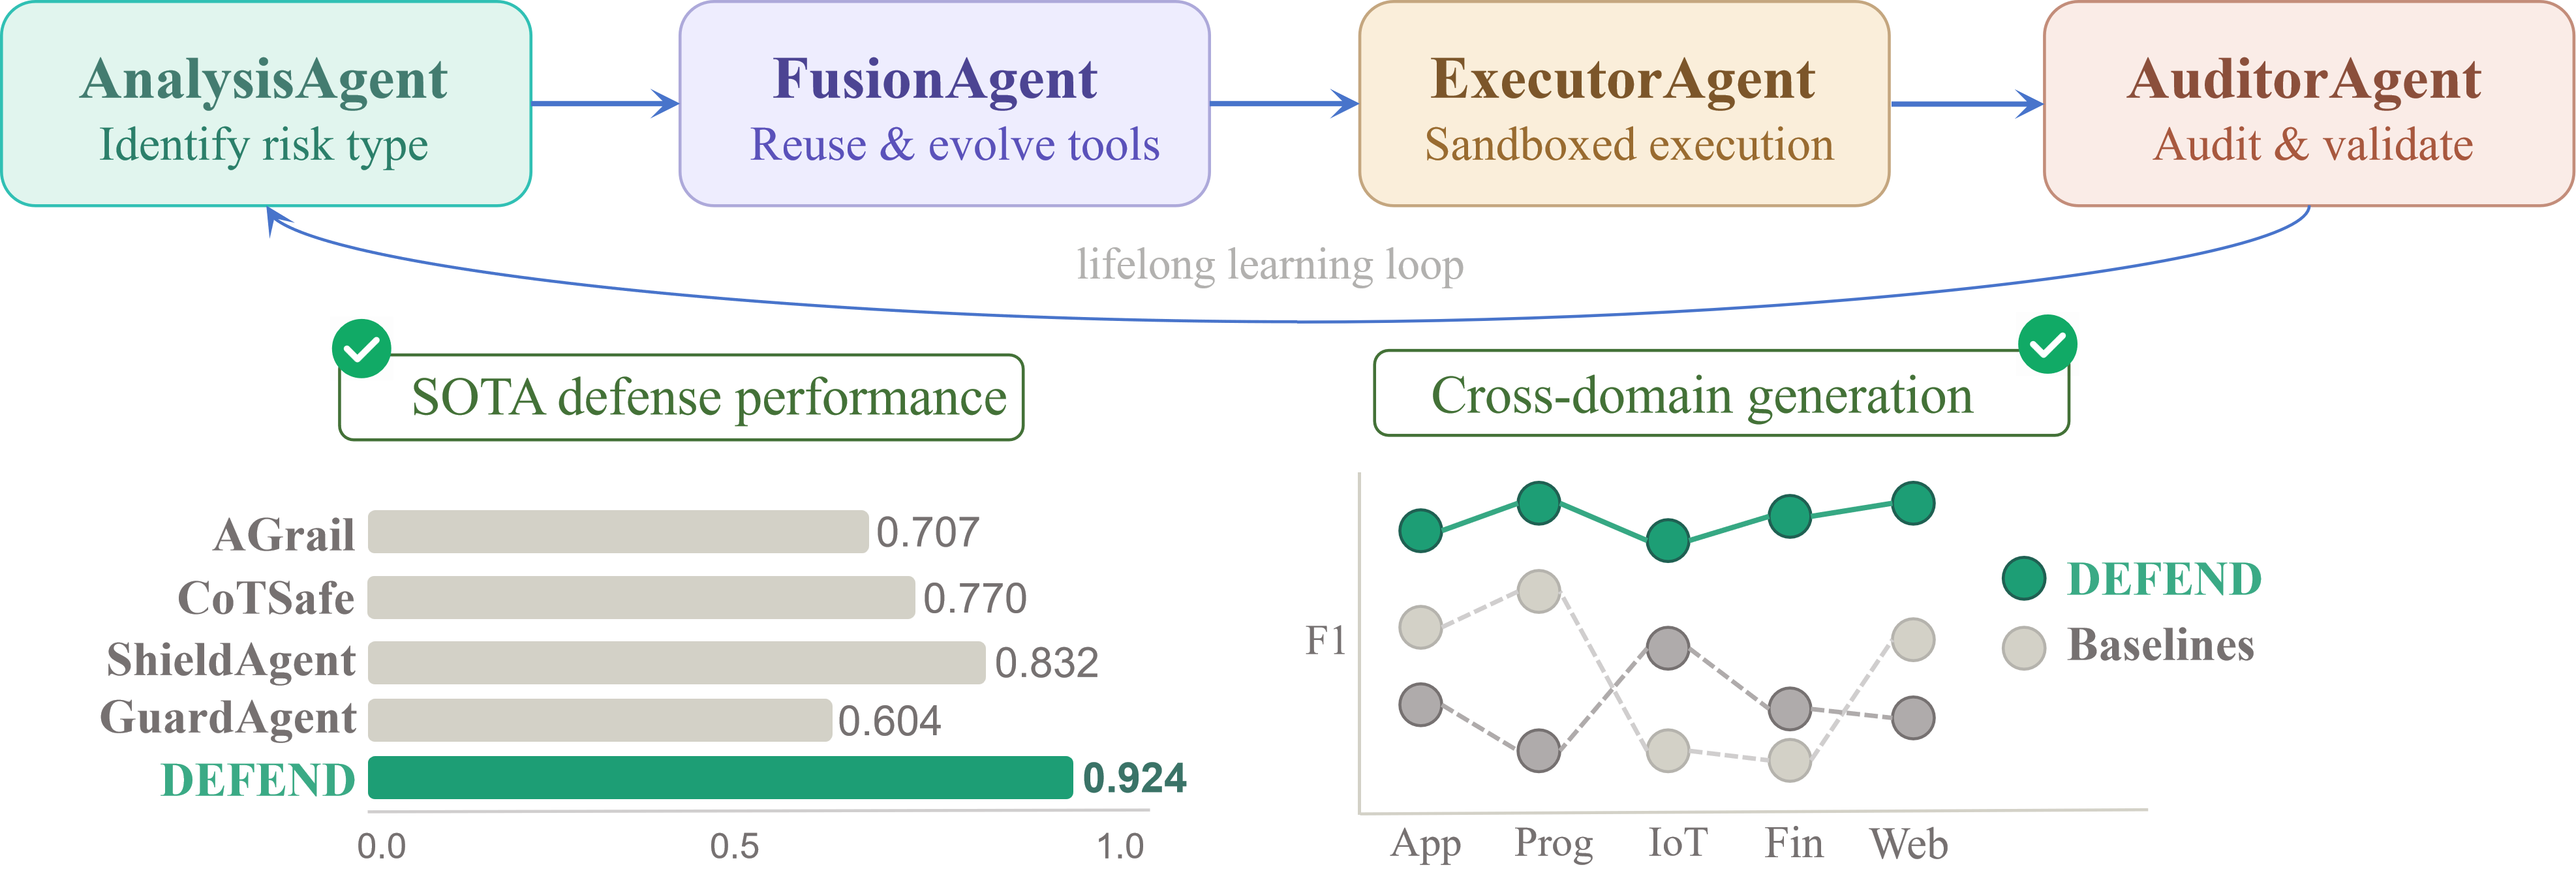
\includegraphics[width=\linewidth]{code/new_intro.png}
%     \caption{Brief introduction to the EVOLVE framework.}
%     \label{fig:intro}
% \end{figure}

%Building safe and reliable intelligent agents represents a core challenge in the pursuit of Artificial General Intelligence (AGI)~\citep{fang2025comprehensivesurveyselfevolvingai}. In recent years, significant progress has been made in intelligent agents driven primarily by large language models (LLMs)~\citep{gao2025evovlesurvey}. These agents are capable of autonomously managing files, invoking tools, and interacting with their environments, leading to widespread application across various aspects of daily life~\citep{yu2025finmem,yang2024llmpsychology,gur2023webagent}. Nevertheless, the continuous expansion of their capabilities broadens the width for agent security. For instance, a medical agent could misuse permissions to leak patient data~\citep{yuan2024rjudge}, while an autonomous driving agent might misinterpret user instructions and execute dangerous maneuvers~\citep{han2025dme,mao2023driving}. Establishing effective safety mechanisms for LLM-based agents has thus become a pressing imperative.

%Current defense mechanisms, however, remain fundamentally static. Prompt-based methods such as CoTSafe~\citep{yin2024safeagentbench} rely on the inherent ambiguity of natural language reasoning. Model-based approaches~\citep{zhang2024asb} employ fine-tuned discriminators whose performance is tightly coupled to training distributions. Rule or knowledge-based frameworks~\citep{xiang2024guardagent,sadhu2024athena} encode a priori human knowledge into fixed safety guidelines that cannot scale to emerging domains. These approaches share a common fragility: they generalize poorly under distributional shift~\citep{shahriar2025survey}. In our experiments, representative baselines exhibit performance fluctuations of up to 65\% across benchmarks, confirming that static defenses are structurally inadequate for the open-world environments in which agents operate.

%This fragility points to a deeper structural mismatch. Real-world risks are open-ended and emergent, yet existing defenses assume a closed threat space that can be enumerated in advance. Overcoming this mismatch demands a paradigm shift: defense itself must become a dynamic, evolving capability rather than a fixed policy. The inspiration comes from how human institutions develop resilience---not by memorizing every known threat, but by continuously abstracting patterns from experience, refining response strategies, and forming transferable coping mechanisms~\citep{cai2025building}. Such cumulative adaptive processes are precisely what static frameworks lack.


%Here we present EVOLVE (\underline{EVO}lving \underline{L}ifelong-learning agent defense \underline{V}ia audited cod\underline{E} tools), a self-evolving security framework that continuously generates, reuses, audits, and refines executable guardrail tools through lifelong interaction. The core insight is to treat defense not as a fixed set of rules or natural language constraints, but as an evolving security capability codified in executable Python tools. EVOLVE operates through four coordinated agents: AnalysisAgent dynamically identifies emerging risks and generates targeted guardrail tools by reasoning over a lifelong risk knowledge library; FusionAgent retrieves semantically similar tools and fuses them with new ones, enabling cross-domain reuse and continuous evolution; ExecutorAgent safely executes both guardrail tools and agent operations within a sandboxed environment, producing verifiable execution evidence; and AuditorAgent independently audits tool integrity and synthesizes full-pipeline signals to deliver final security verdicts, forming an autonomous closed loop from risk perception through tool evolution to trusted verification.


%\vspace{-1mm}
\begin{chapquote}{Charles Darwin}
``It is not the strongest of the species that survives, nor the most intelligent, but the one most responsive to change.''  
\end{chapquote}  
%\vspace{-5mm}


Large language model (LLM)-driven agents are rapidly emerging as a central pathway toward Artificial General Intelligence (AGI). These LLM agents can autonomously invoke tools, execute actions, interact with external environments, and continuously adapt their behavior through feedback and memory~\citep{fang2025comprehensivesurveyselfevolvingai,gao2025evovlesurvey}, enabling their deployment across increasingly high-stakes domains ~\citep{yu2025finmem,yang2024llmpsychology,gur2023webagent}. As agents transition from passive language interfaces to active decision-making systems operating in open-world environments, agents' safety risks may lead not only to harmful outputs, but also to severe real-world consequences such as financial fraud, privacy leakage, unsafe robotic actions, and hazardous autonomous behaviors~\citep{yuan2024rjudge,han2025dme,mao2023driving}. Ensuring the safety and trustworthiness of LLM agents has therefore become a critical challenge for the future of intelligent systems.

To mitigate these risks, existing defense frameworks have introduced various forms of safety guardrails, including prompt-based reasoning constraints~\citep{yin2024safeagentbench}, fine-tuned safety discriminators~\citep{zhang2024asb}, and rule- or knowledge-driven policy enforcement~\citep{xiang2024guardagent,sadhu2024athena}. Despite their methodological differences, these approaches share a common assumption: that risks can be predefined in advance and mitigated through static protection policies. However, real-world environments are inherently open-ended and continuously evolving. Emerging risks frequently arise outside predefined safety distributions, causing existing defenses to to degrade as threat scenarios shift~\citep{shahriar2025survey}. This reveals a fundamental structural mismatch between dynamic risks and static defenses.

Overcoming this mismatch requires rethinking the nature of defense itself. In human societies, resilience to emerging risks does not arise from memorizing every possible threat, but from cumulative adaptive processes that continuously abstract patterns from experience, refine coping strategies, and iteratively verify newly acquired knowledge~\citep{boyd1988culture,henrich2015secret,weick2011managing,taleb2012things}. Research in cultural evolution, organizational adaptation, and collective intelligence suggests that robust systems emerge through ongoing cycles of exploration, refinement, reuse, and institutional auditing rather than fixed rule preservation~\cite{argyris1997organizational}. By contrast, most existing agent defense frameworks remain fundamentally static, lacking the ability to continuously evolve their protection mechanisms in response to changing environments. This motivates a central question: \emph{can agent defense itself become a self-evolving capability?}


Here we present EVOLVE, a self-evolving defense framework for LLM agents that reformulates agent safety as a process of \emph{cumulative security evolution} through executable guardrail tools, shown in Figure~\ref{fig:Pipeline}. Inspired by how human societies build resilience to emerging risks, EVOLVE organizes defense into four adaptive stages: \emph{generation}, which externalizes newly discovered risks into executable guardrail tools; \emph{reuse}, which retrieves and fuses previously generated tools to accumulate transferable security knowledge; \emph{audit}, which independently verifies evolved tools before they can participate in future defense processes; and \emph{refinement}, which iteratively repairs unsafe tools and replans unsafe agent behaviors through feedback. These stages are instantiated by a set of specialized agents that collectively establish an autonomous closed loop from risk perception to trusted adaptation. Together, EVOLVE enables security knowledge to be accumulated, governed, and continuously improved throughout lifelong interaction, allowing defense systems to evolve alongside changing environments while remaining bounded by verifiable safety constraints.

Extensive experiments across 3 agent safety benchmarks (RJudge~\cite{yuan2024rjudge}, ASSEBench~\cite{luo2025agentauditor}, AgentHarm~\cite{andriushchenko2025agentharm}) and 4 backbone LLMs (DeepSeek~\cite{liu2024deepseek}, GPT~\cite{achiam2023gpt}, Claude~\cite{bai2022constitutional}, Gemini~\cite{team2023gemini}) demonstrate that EVOLVE consistently outperforms existing defense frameworks largely (+22\% average F1 score compared with the runner-up) across open-world risk scenarios. Besides, we further validate EVOLVE in embodied agent scenarios in the AI2THOR environment \cite{kolve2022ai2thor}, a 6-DoF robotic arm~\cite{elephant}, and a real-world tool-calling agent handling financial operations (OpenClaw~\cite{openclaw}), demonstrating that the framework generalizes from text-based benchmarks to real-world deployment. Notably, the framework achieves high rates of guardrail tool reuse and iterative refinement (up to 86\%), indicating that security knowledge can accumulate and evolve through interaction rather than remaining fixed after deployment.

By integrating lifelong self-evolution with agent defense, EVOLVE shifts agent security from static policy enforcement toward continuously adaptive protection mechanisms. Our findings suggest that scalable safety for future intelligent agents may depend not on enumerating all possible risks in advance, but on enabling defense systems themselves to expand, audit, and compound their security capabilities through tool-level inheritance.
%Extensive experiments across three benchmarks spanning finance, healthcare, industry, and other domains, with four backbone LLMs, demonstrate that EVOLVE consistently outperforms all baselines under substantial distribution shifts, achieving F1 scores stably between 0.86 and 0.92 while static baselines exhibit performance variations of up to 20\% across benchmarks. A tool reuse rate exceeding 50\% confirms the framework's capacity for continuous self-optimization through interaction. We further validate EVOLVE in embodied intelligence scenarios (AI2THOR), a 6-DoF robotic arm, and an autonomous digital agent, demonstrating that the framework generalizes from text-based benchmarks to both physical and real-world deployment.

%By being the first to integrate agent security with agent self-evolution, EVOLVE breaks through the limitations of traditional static defense baselines and demonstrates exceptional defensive capabilities. As a pioneering effort toward unification in the field of agent defense, our findings indicate that codifying security policies as auditable, executable artifacts, rather than fixed rules or natural language constraints, is key to bridging the generalization gap and achieving universal agent protection.
% \begin{figure}
%     \centering
%     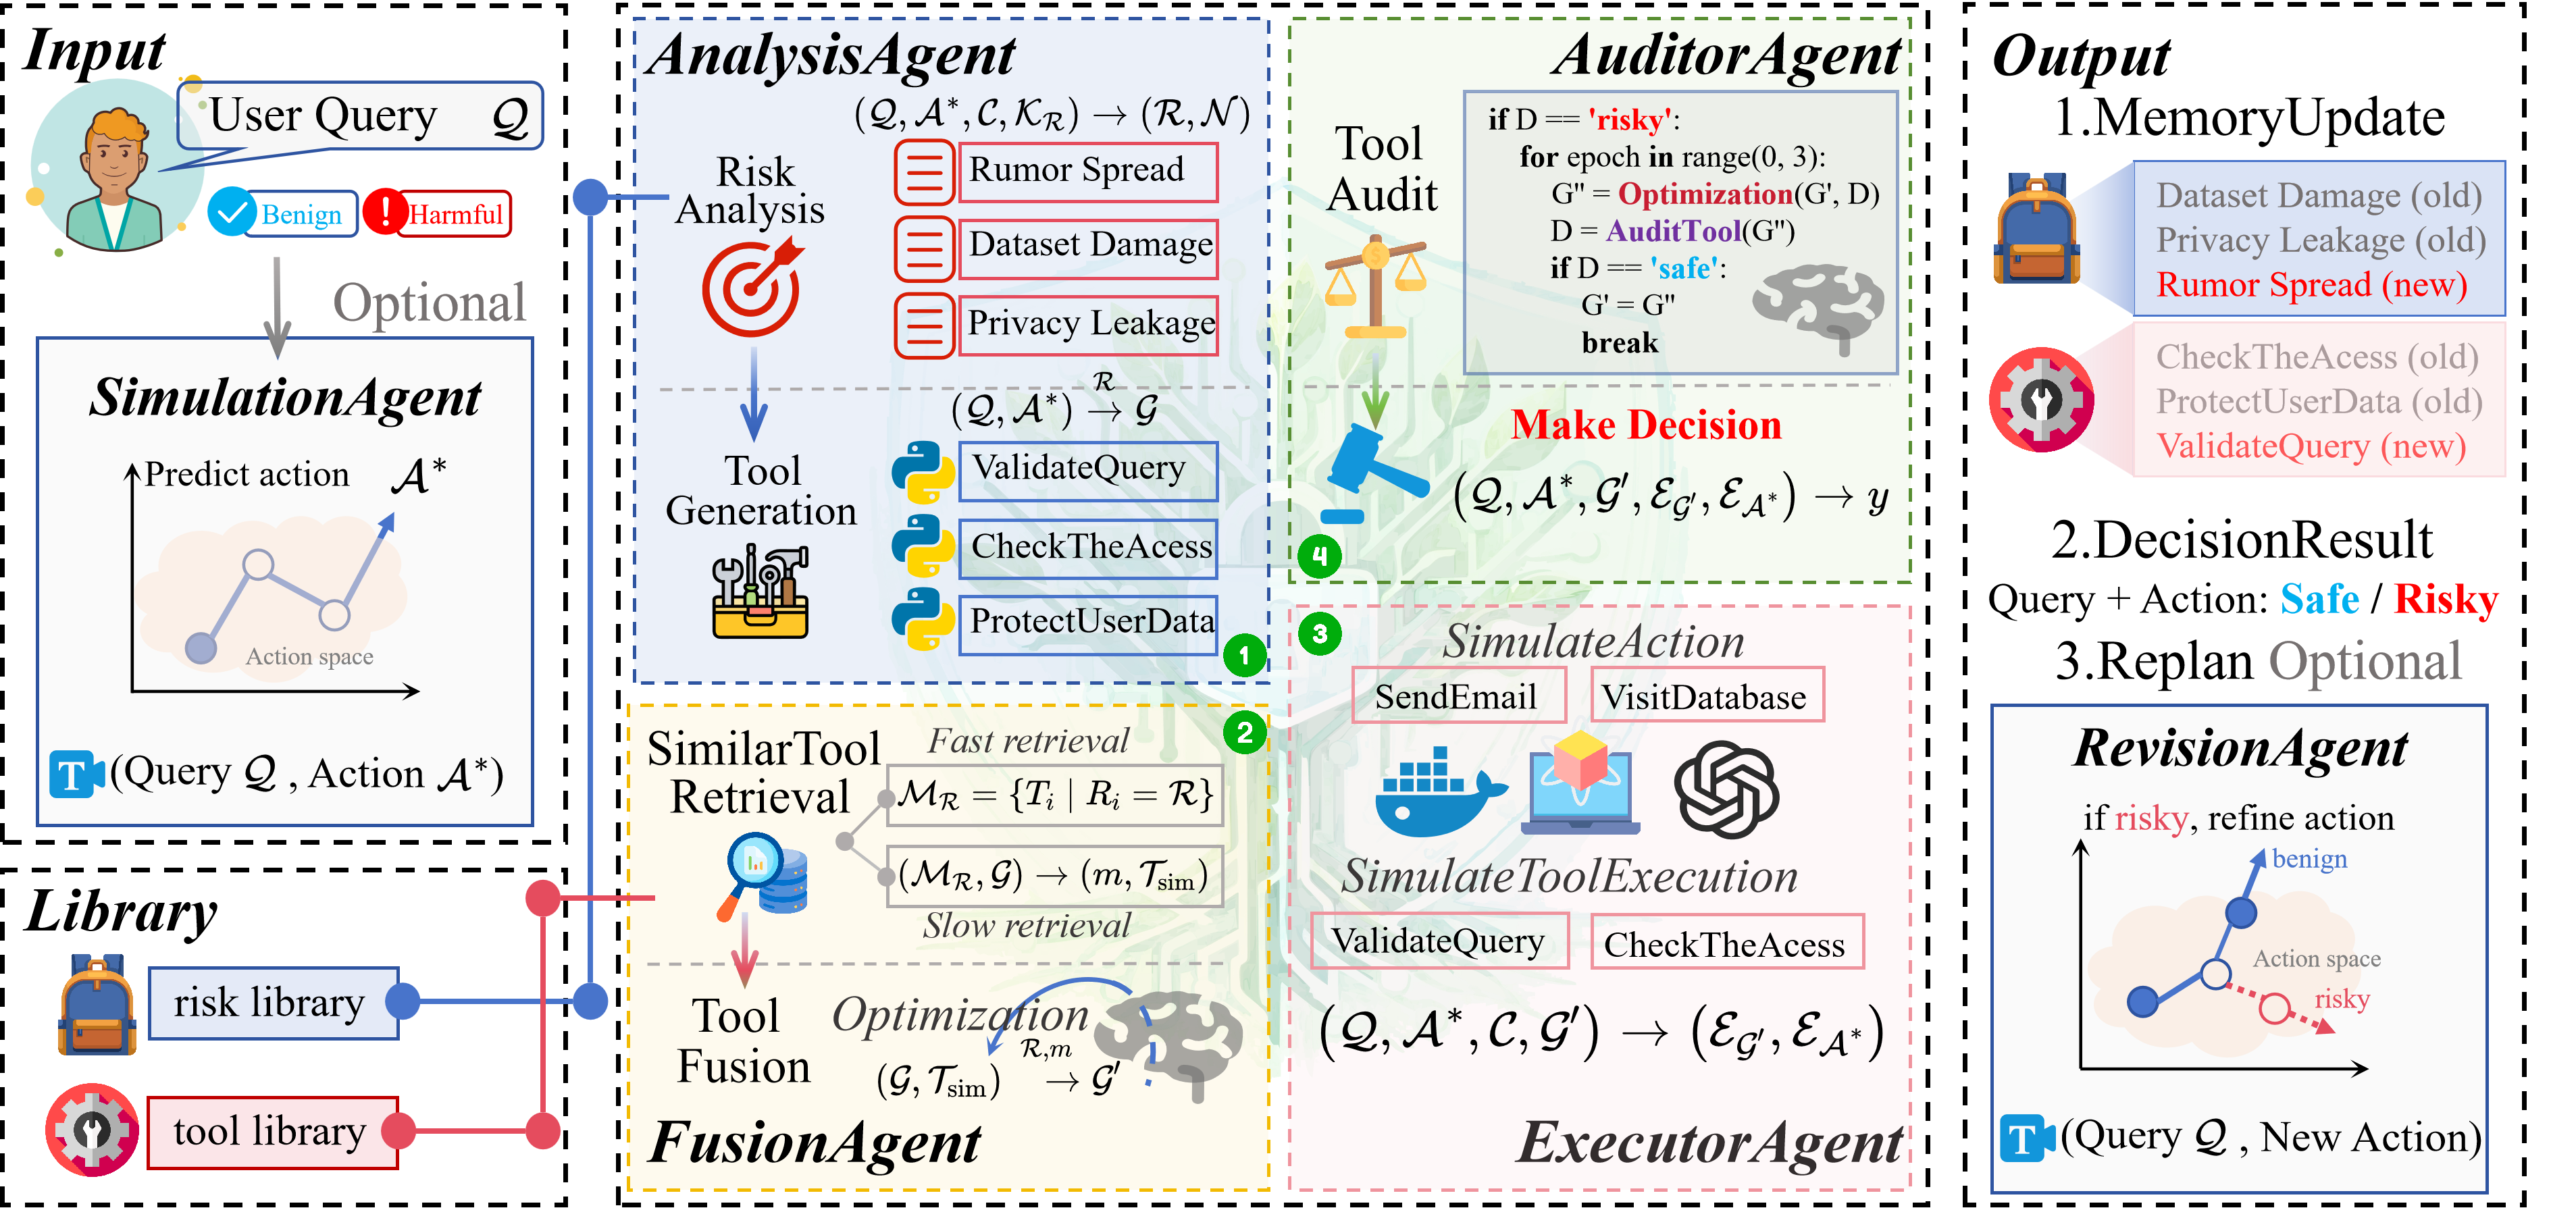
\includegraphics[width=\linewidth]{code/pipeline.png}
%     \caption{EVOLVE's framework.}
%     \label{fig:Pipeline}
% \end{figure}

\begin{figure*}[!t]
      \centering
      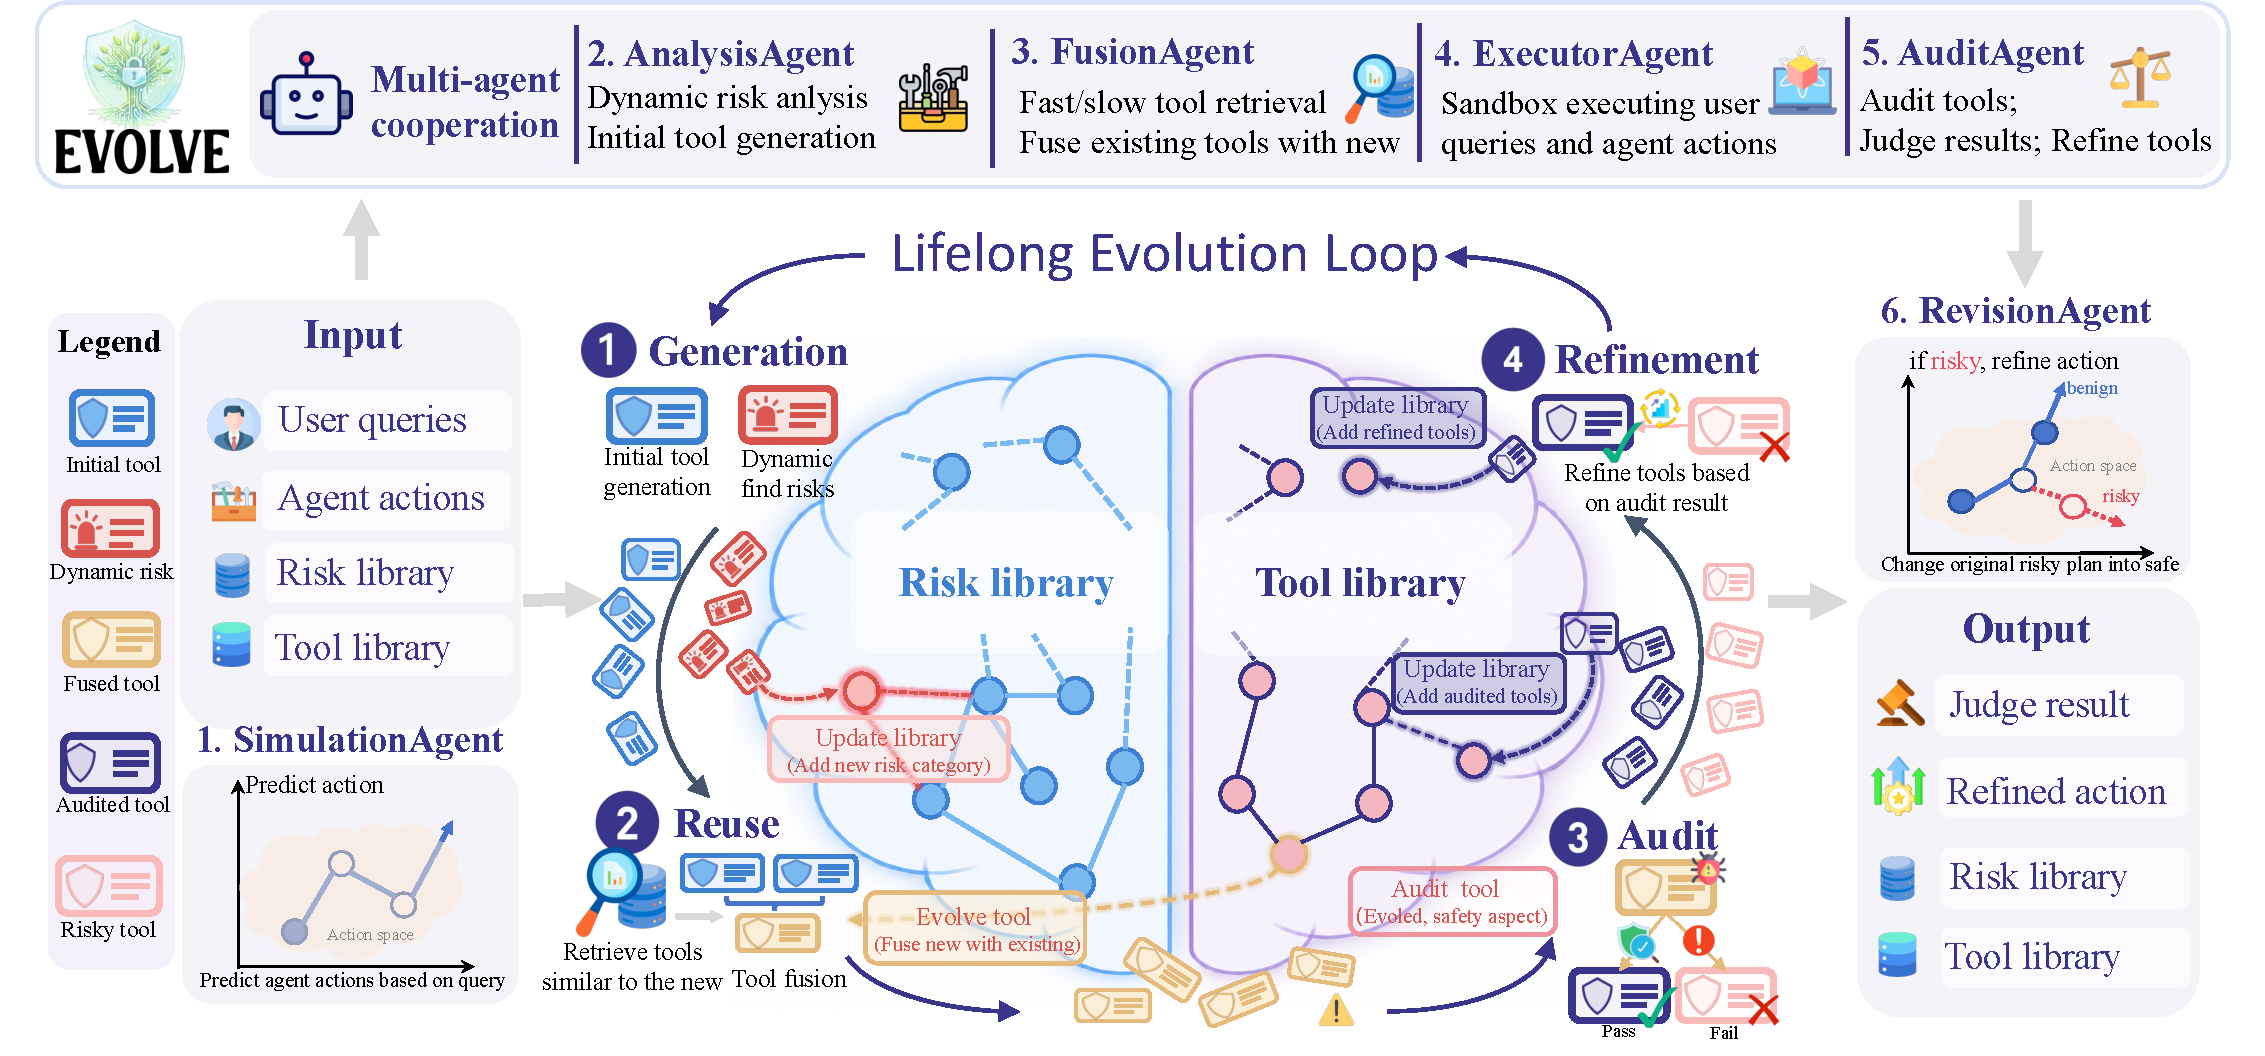
\includegraphics[width=\linewidth]{code/framework.pdf}
      \caption{EVOLVE's framework. The four-stage pipeline---generation, reuse, audit, and refinement---mirrors the cumulative adaptive cycle through which human institutions develop resilience to evolving risks.}
      \label{fig:Pipeline}
  \end{figure*}